\documentclass{article}%
\usepackage[T1]{fontenc}%
\usepackage[utf8]{inputenc}%
\usepackage{lmodern}%
\usepackage{textcomp}%
\usepackage{lastpage}%
\usepackage{geometry}%
\geometry{margin=0.5in,headheight=10pt,footskip=0.2in,tmargin=0.5in,bmargin=0.5in}%
\usepackage{graphicx}%
\usepackage{float}%
\usepackage{booktabs}%
\usepackage{hyperref}%
\usepackage{caption}%
\usepackage{subcaption}%
\usepackage{ragged2e}%
%
\title{Analysis Report}%
\author{AutoPrep}%
\date{\today}%
%
\begin{document}%
\normalsize%
\maketitle%

                \begin{abstract}
                This raport has been generated with AutoPrep using
                \end{abstract}
            %
\tableofcontents%
\newpage%
\section{Overview}%
\label{sec:Overview}%

%
\subsection{System}%
\label{subsec:System}%

%


\begin{table}[H]%
\begin{center}%
\begin{tabular}{l r}%
\hline%
System&Darwin\\%
Machine&arm64\\%
Processor&arm\\%
Architecture&64bit\\%
Python Version&3.11.10\\%
Physical Cores&8\\%
Logical Cores&8\\%
CPU Frequency (MHz)&4056\\%
Total RAM (GB)&16.0000\\%
Available RAM (GB)&4.4831\\%
Total Disk Space (GB)&460.4317\\%
Free Disk Space (GB)&263.8063\\%
\hline%
\end{tabular}%
\end{center}%
\end{table}

%
\subsection{Dataset}%
\label{subsec:Dataset}%

%


\begin{table}[H]%
\begin{center}%
\begin{tabular}{l r}%
\hline%
Number of samples&1309\\%
Number of features&13\\%
Numeric features&6\\%
Categorical features&7\\%
\hline%
\end{tabular}%
\end{center}%
\end{table}

%
\subsection{Target Distribution}%
\label{subsec:TargetDistribution}%

%


\begin{table}[H]%
\begin{center}%
\begin{tabular}{l r}%
\hline%
\textbf{Category}&\textbf{Value}\\%
\hline%
0&809\\%
1&500\\%
\hline%
\end{tabular}%
\end{center}%
\caption{Target Distribution}%
\end{table}

%


\begin{figure}[H]%
\centering%
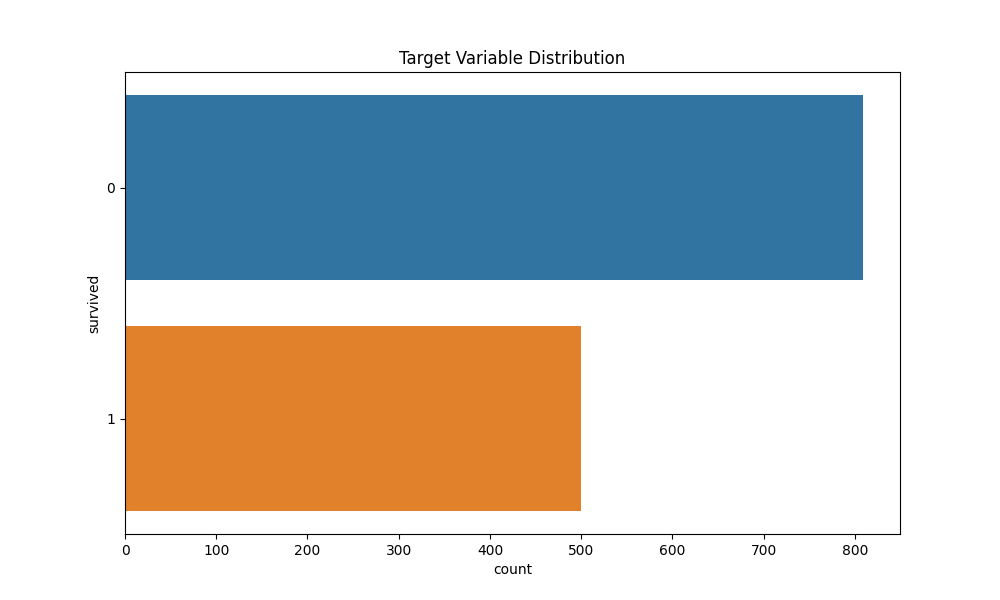
\includegraphics[width=0.9\textwidth]{/Users/pawelp/Desktop/education/pw/automl/AutoPrep/examples/reports/figures/target_distribution.png}%
\caption{Target Variable Distribution}%
\end{figure}

%
\subsection{Missing Values}%
\label{subsec:MissingValues}%

%


\begin{table}[H]%
\begin{center}%
\begin{tabular}{l r}%
\hline%
\textbf{Category}&\textbf{Value}\\%
\hline%
pclass&0\\%
survived&0\\%
name&0\\%
sex&0\\%
age&263\\%
sibsp&0\\%
parch&0\\%
ticket&0\\%
fare&1\\%
cabin&1014\\%
embarked&2\\%
boat&823\\%
body&1188\\%
home\_\_dest&564\\%
\hline%
\end{tabular}%
\end{center}%
\caption{Missing Values}%
\end{table}

%


\begin{figure}[H]%
\centering%
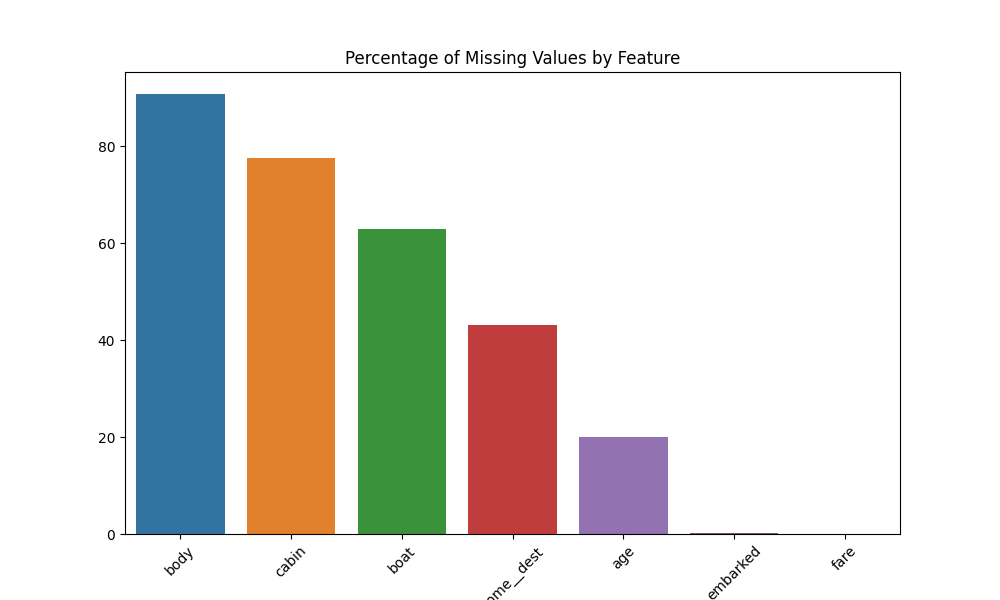
\includegraphics[width=0.9\textwidth]{/Users/pawelp/Desktop/education/pw/automl/AutoPrep/examples/reports/figures/missing_values.png}%
\caption{Missing Values Analysis}%
\end{figure}

%
\section{Exploratory Data Analysis}%
\label{sec:ExploratoryDataAnalysis}%
Visual analysis of the dataset features.

%
\subsection{Numeric Features}%
\label{subsec:NumericFeatures}%

%


\begin{figure}[H]%
\centering%
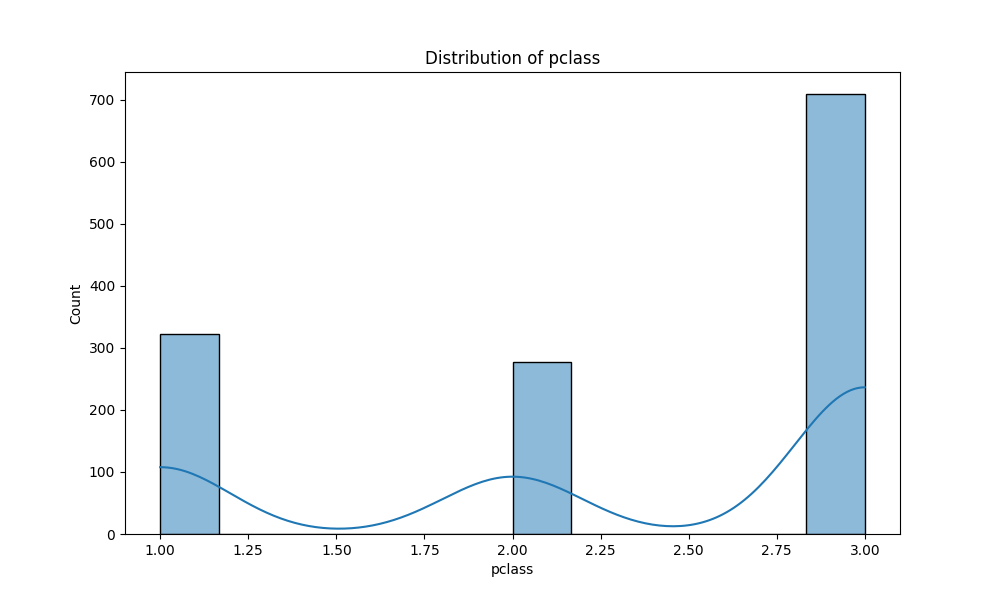
\includegraphics[width=0.9\textwidth]{/Users/pawelp/Desktop/education/pw/automl/AutoPrep/examples/reports/figures/dist_pclass.png}%
\caption{Distribution of pclass}%
\end{figure}

%


\begin{figure}[H]%
\centering%
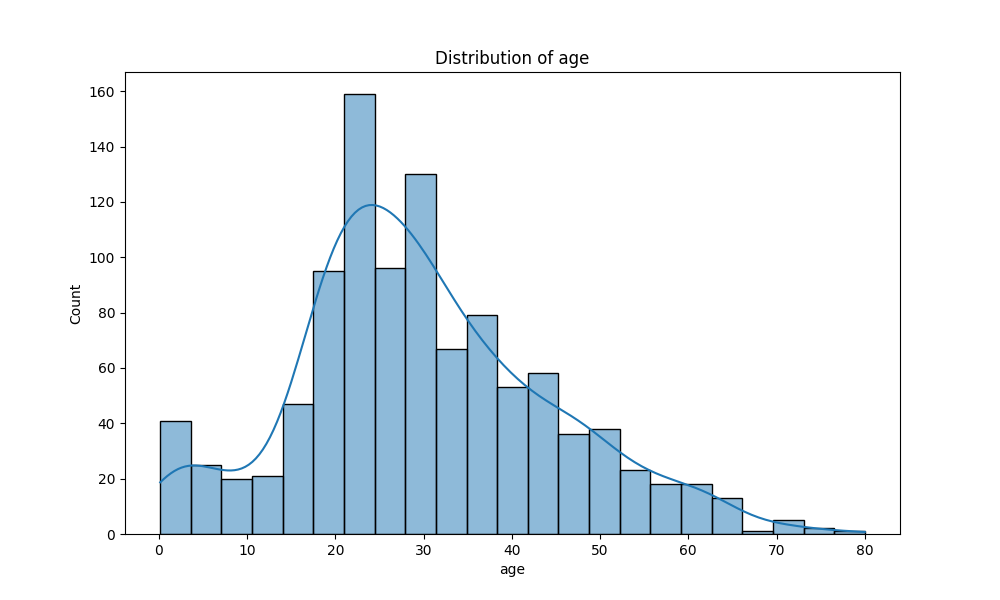
\includegraphics[width=0.9\textwidth]{/Users/pawelp/Desktop/education/pw/automl/AutoPrep/examples/reports/figures/dist_age.png}%
\caption{Distribution of age}%
\end{figure}

%


\begin{figure}[H]%
\centering%
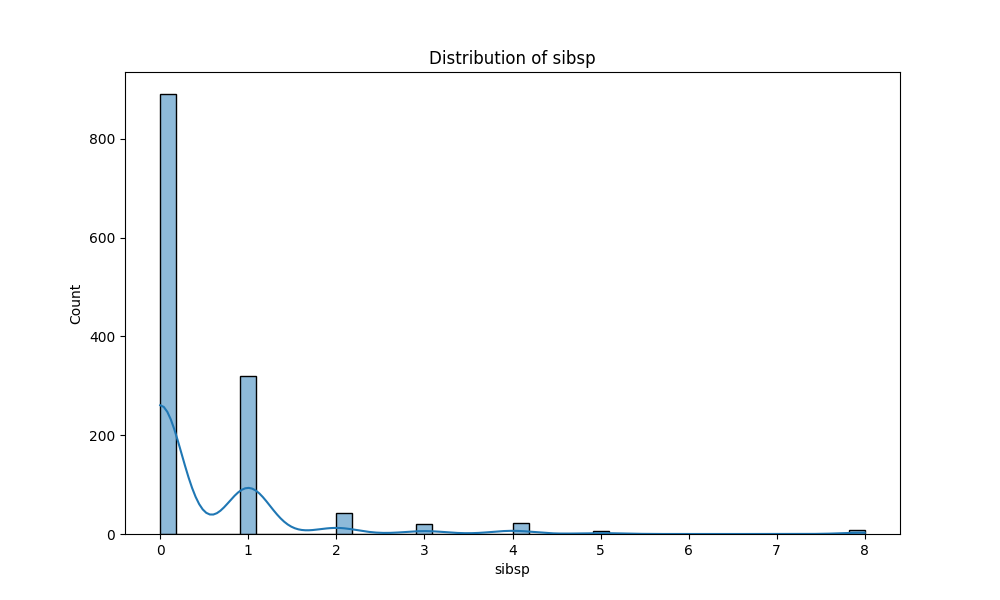
\includegraphics[width=0.9\textwidth]{/Users/pawelp/Desktop/education/pw/automl/AutoPrep/examples/reports/figures/dist_sibsp.png}%
\caption{Distribution of sibsp}%
\end{figure}

%


\begin{figure}[H]%
\centering%
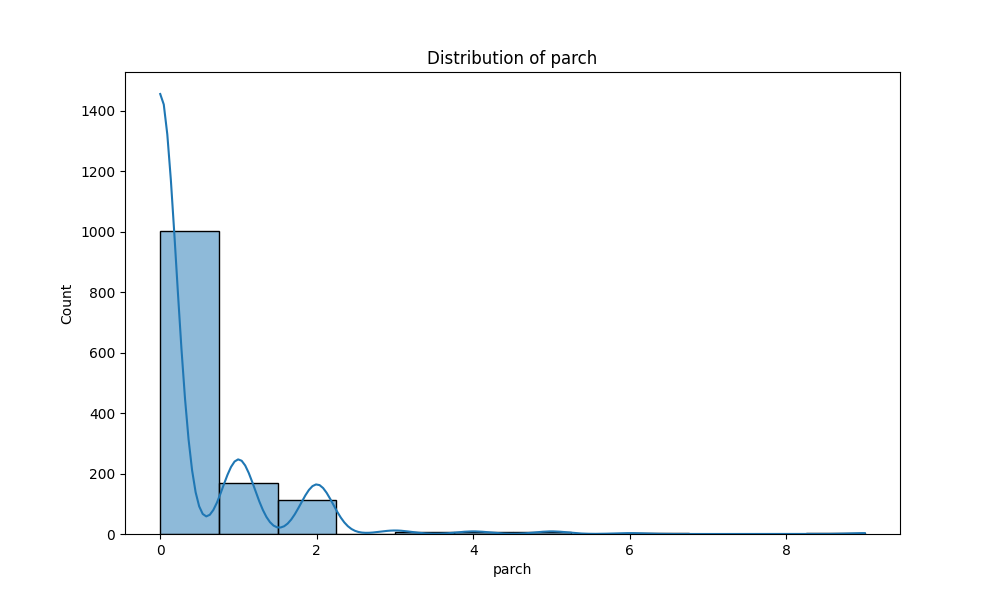
\includegraphics[width=0.9\textwidth]{/Users/pawelp/Desktop/education/pw/automl/AutoPrep/examples/reports/figures/dist_parch.png}%
\caption{Distribution of parch}%
\end{figure}

%


\begin{figure}[H]%
\centering%
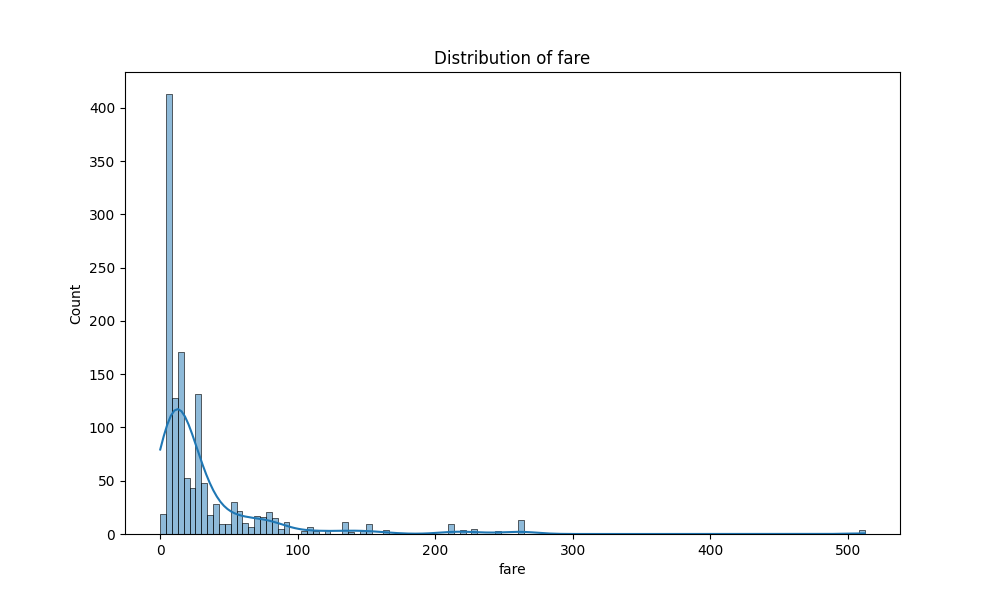
\includegraphics[width=0.9\textwidth]{/Users/pawelp/Desktop/education/pw/automl/AutoPrep/examples/reports/figures/dist_fare.png}%
\caption{Distribution of fare}%
\end{figure}

%


\begin{figure}[H]%
\centering%
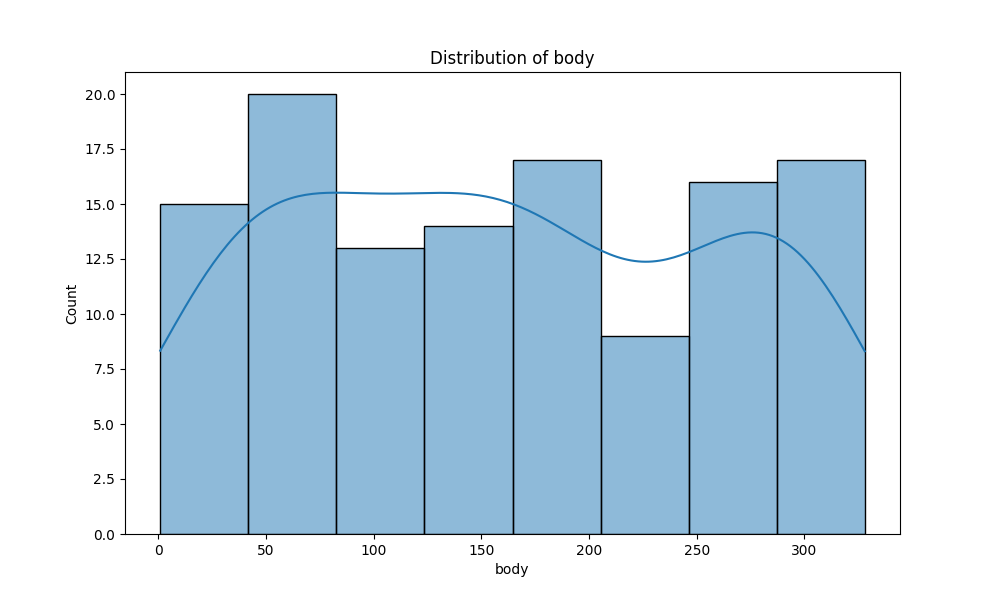
\includegraphics[width=0.9\textwidth]{/Users/pawelp/Desktop/education/pw/automl/AutoPrep/examples/reports/figures/dist_body.png}%
\caption{Distribution of body}%
\end{figure}

%
\subsection{Categorical Features}%
\label{subsec:CategoricalFeatures}%

%


\begin{figure}[H]%
\centering%
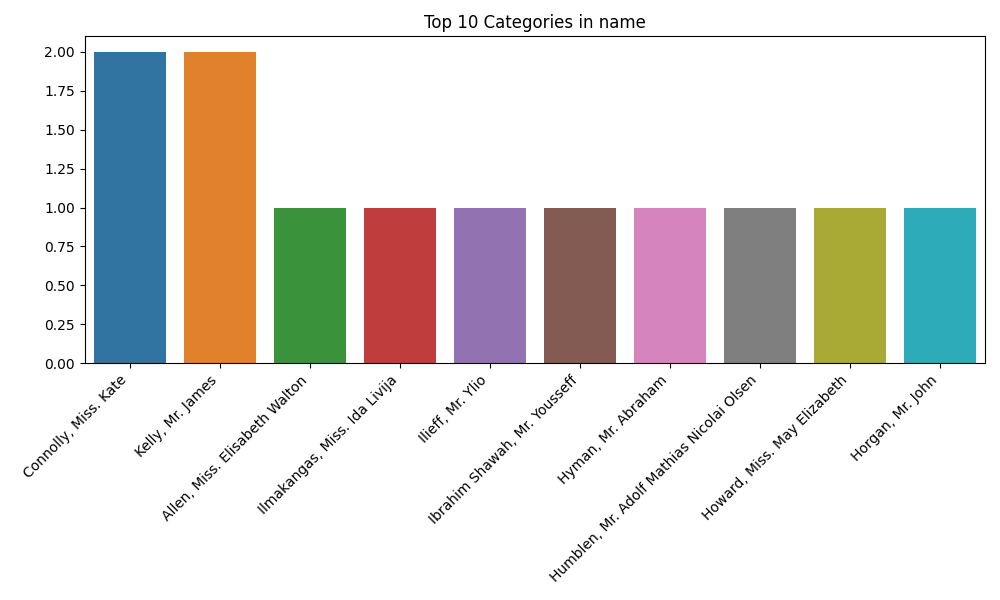
\includegraphics[width=0.9\textwidth]{/Users/pawelp/Desktop/education/pw/automl/AutoPrep/examples/reports/figures/cat_name.png}%
\caption{Distribution of name}%
\end{figure}

%


\begin{figure}[H]%
\centering%
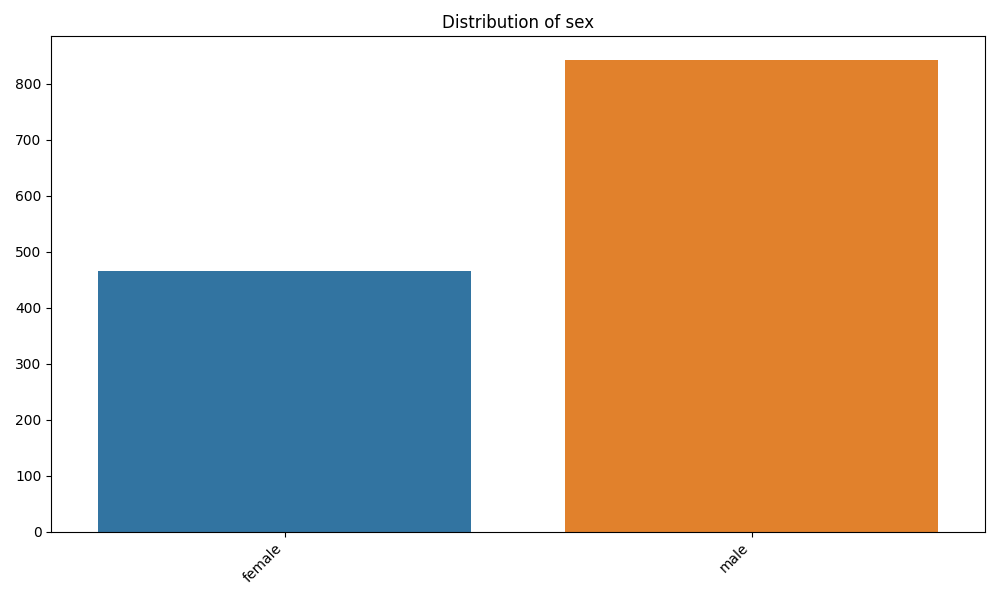
\includegraphics[width=0.9\textwidth]{/Users/pawelp/Desktop/education/pw/automl/AutoPrep/examples/reports/figures/cat_sex.png}%
\caption{Distribution of sex}%
\end{figure}

%


\begin{figure}[H]%
\centering%
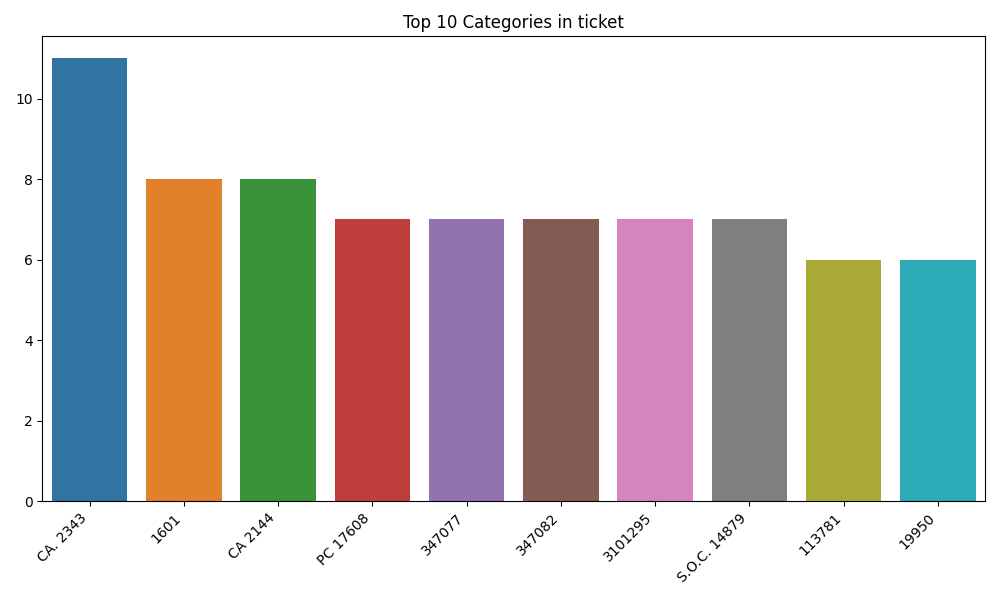
\includegraphics[width=0.9\textwidth]{/Users/pawelp/Desktop/education/pw/automl/AutoPrep/examples/reports/figures/cat_ticket.png}%
\caption{Distribution of ticket}%
\end{figure}

%


\begin{figure}[H]%
\centering%
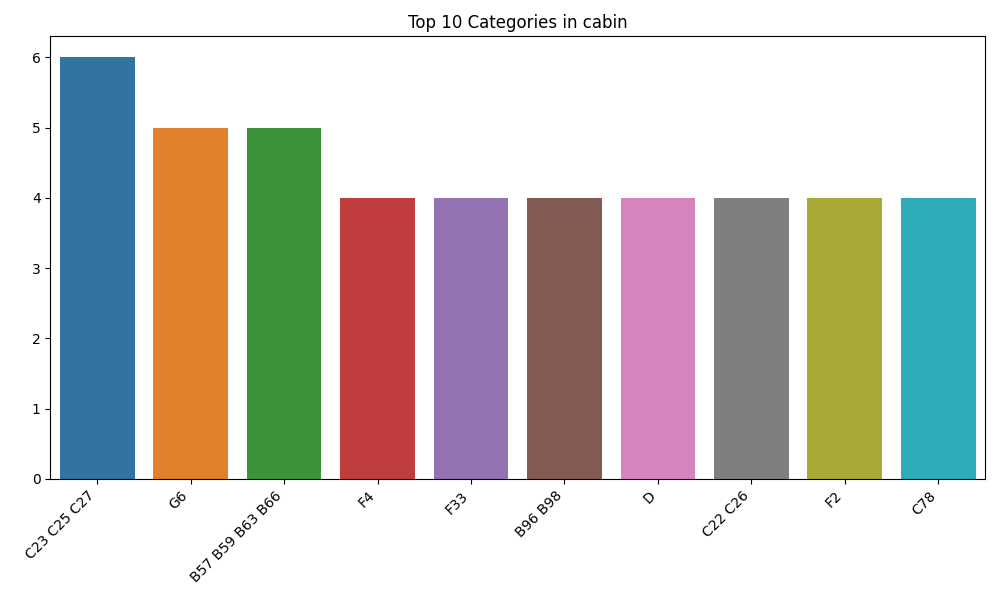
\includegraphics[width=0.9\textwidth]{/Users/pawelp/Desktop/education/pw/automl/AutoPrep/examples/reports/figures/cat_cabin.png}%
\caption{Distribution of cabin}%
\end{figure}

%


\begin{figure}[H]%
\centering%
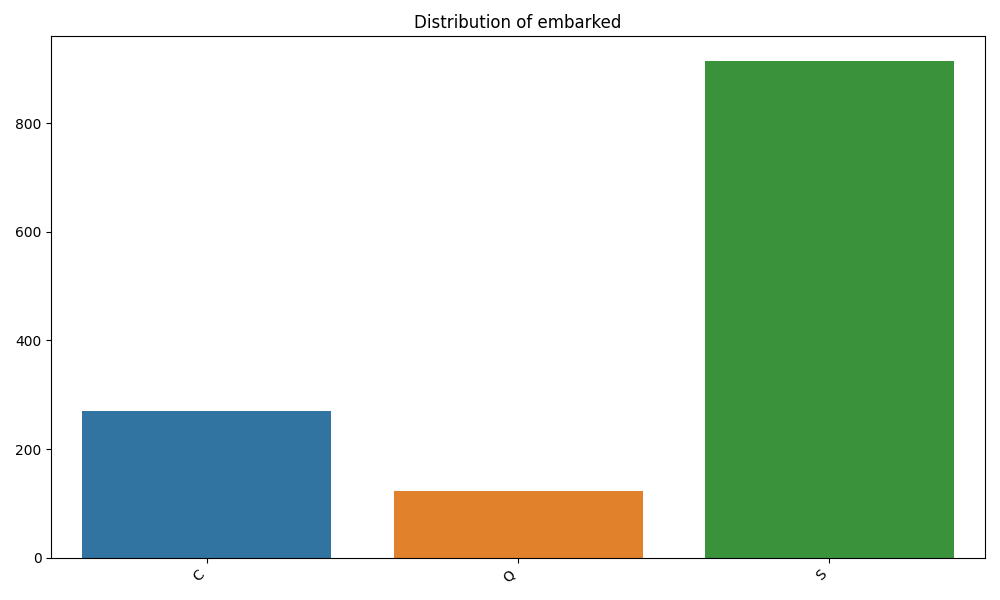
\includegraphics[width=0.9\textwidth]{/Users/pawelp/Desktop/education/pw/automl/AutoPrep/examples/reports/figures/cat_embarked.png}%
\caption{Distribution of embarked}%
\end{figure}

%


\begin{figure}[H]%
\centering%
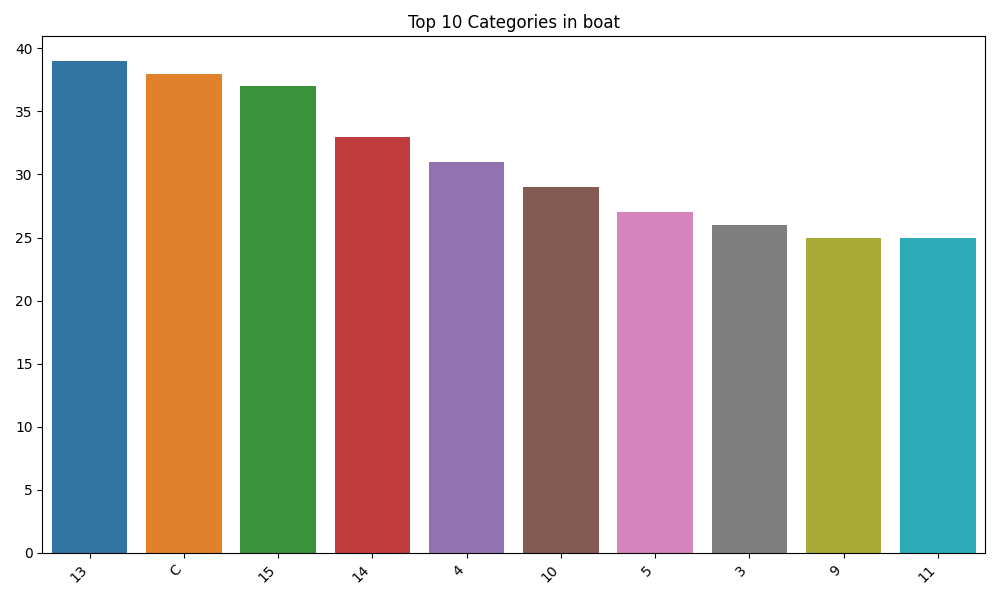
\includegraphics[width=0.9\textwidth]{/Users/pawelp/Desktop/education/pw/automl/AutoPrep/examples/reports/figures/cat_boat.png}%
\caption{Distribution of boat}%
\end{figure}

%


\begin{figure}[H]%
\centering%
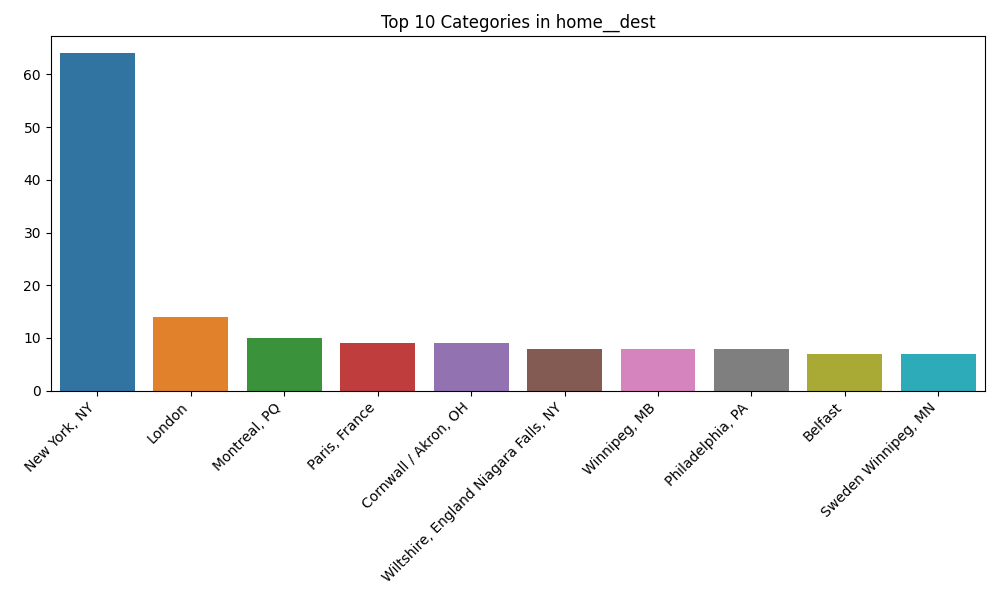
\includegraphics[width=0.9\textwidth]{/Users/pawelp/Desktop/education/pw/automl/AutoPrep/examples/reports/figures/cat_home__dest.png}%
\caption{Distribution of home\_\_dest}%
\end{figure}

%
\subsection{Correlation Analysis}%
\label{subsec:CorrelationAnalysis}%

%


\begin{figure}[H]%
\centering%
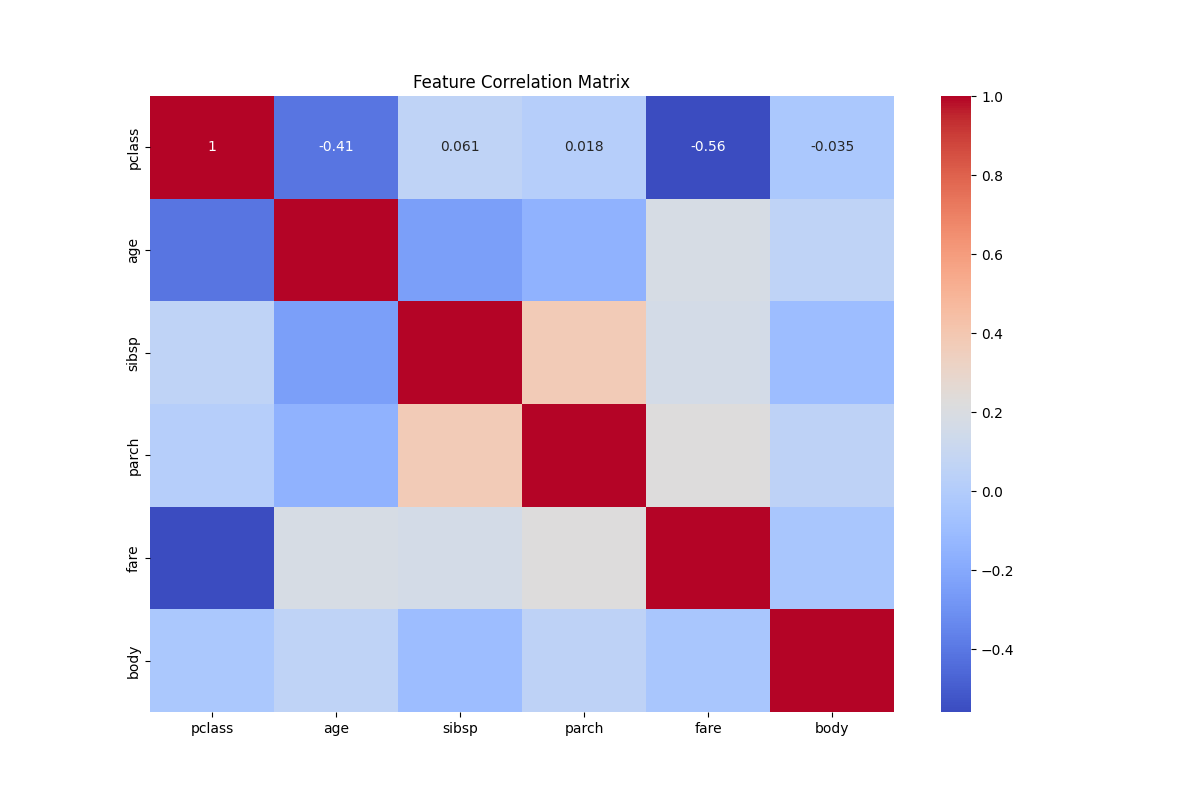
\includegraphics[width=0.9\textwidth]{/Users/pawelp/Desktop/education/pw/automl/AutoPrep/examples/reports/figures/correlation_matrix.png}%
\caption{Feature Correlation Matrix}%
\end{figure}

%


\begin{figure}[H]%
\centering%
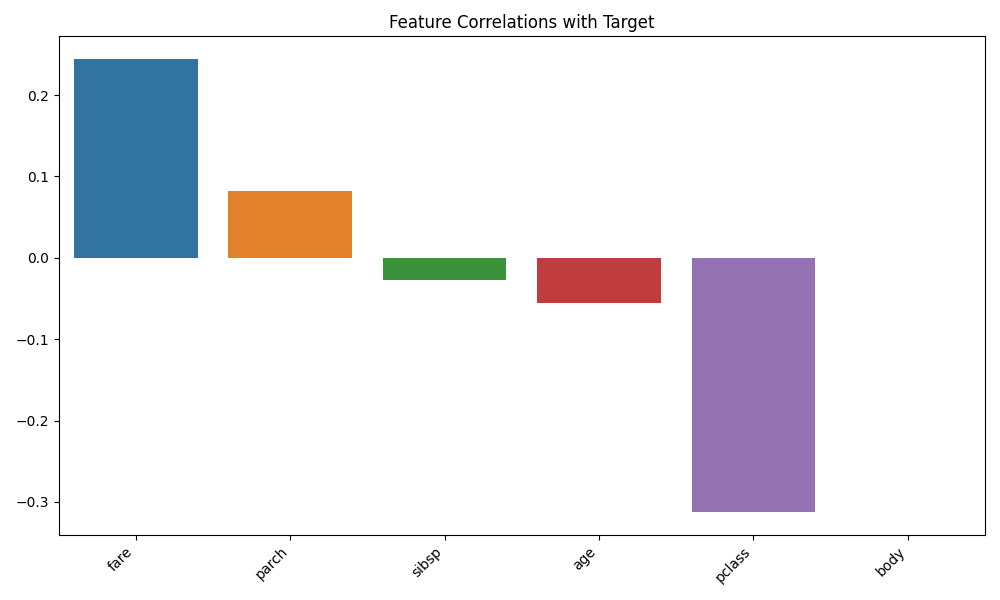
\includegraphics[width=0.9\textwidth]{/Users/pawelp/Desktop/education/pw/automl/AutoPrep/examples/reports/figures/target_correlations.png}%
\caption{Feature Correlations with Target}%
\end{figure}

%
\section{Model Performance}%
\label{sec:ModelPerformance}%

%
\subsection{Cross{-}validation Results}%
\label{subsec:Cross{-}validationResults}%
5-fold CV Score: 0.9761 (+/- 0.0121)

%
\subsection{Test Set Performance}%
\label{subsec:TestSetPerformance}%

%
\begin{verbatim}
              precision    recall  f1-score   support

           0       0.95      1.00      0.98       144
           1       1.00      0.94      0.97       118

    accuracy                           0.97       262
   macro avg       0.98      0.97      0.97       262
weighted avg       0.97      0.97      0.97       262

\end{verbatim}%
\subsection{Confusion Matrix}%
\label{subsec:ConfusionMatrix}%

%


\begin{figure}[H]%
\centering%
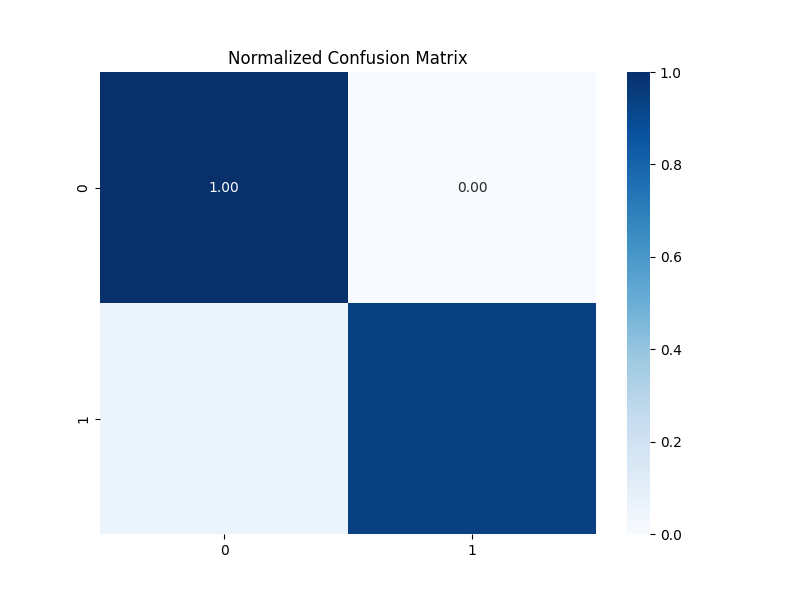
\includegraphics[width=0.9\textwidth]{/Users/pawelp/Desktop/education/pw/automl/AutoPrep/examples/reports/figures/confusion_matrix.png}%
\caption{Normalized Confusion Matrix}%
\end{figure}

%
\section{Feature Importance Analysis}%
\label{sec:FeatureImportanceAnalysis}%
Analysis of feature importance in the model.

%


\begin{figure}[H]%
\centering%
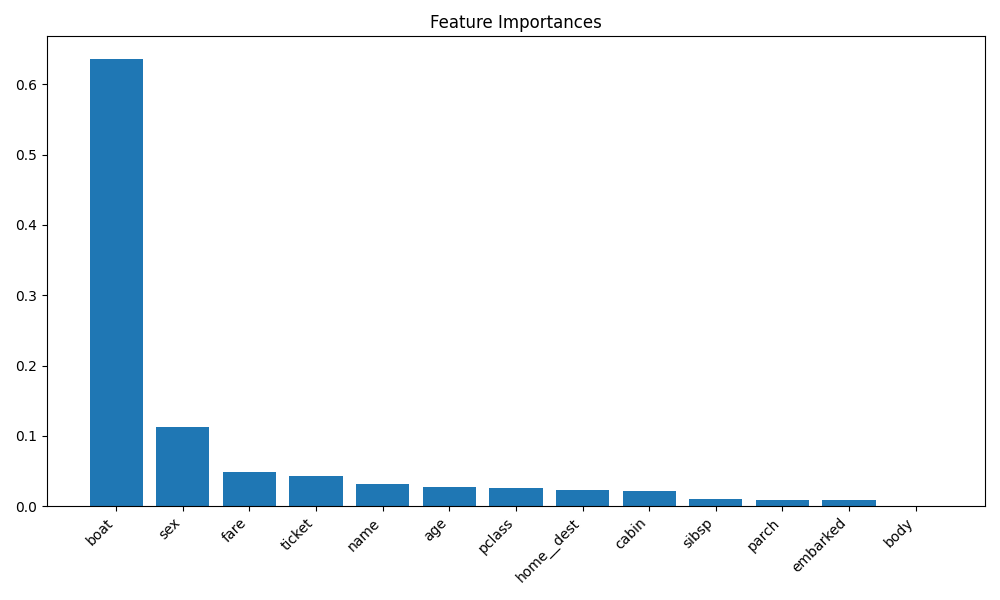
\includegraphics[width=0.9\textwidth]{/Users/pawelp/Desktop/education/pw/automl/AutoPrep/examples/reports/figures/feature_importance.png}%
\caption{Feature Importance Rankings}%
\end{figure}

%
\end{document}
